\documentclass{assignment}
\usepackage{amsmath}
\usepackage{graphicx}
\usepackage{hyperref}
\usepackage{listings}
\usepackage{subcaption}
\usepackage{enumitem}
\usepackage{amssymb}
\usepackage{float}
\lstset{
 numbers=left
}

\newlist{legal}{enumerate}{10}
\setlist[legal]{label*=\arabic*.}

%\DeclareMathSizes{10}{10}{10}{10}


\usepackage{color}

\definecolor{codegreen}{rgb}{0,0.6,0}
\definecolor{codegray}{rgb}{0.5,0.5,0.5}
\definecolor{codepurple}{rgb}{0.58,0,0.82}
\definecolor{backcolour}{rgb}{0.95,0.95,0.92}
 
\lstdefinestyle{mystyle}{
    backgroundcolor=\color{backcolour},   
    commentstyle=\color{codegreen},
    keywordstyle=\color{magenta},
    numberstyle=\tiny\color{codegray},
    stringstyle=\color{codepurple},
    basicstyle=\footnotesize,
    breakatwhitespace=false,         
    breaklines=true,                 
    captionpos=b,                    
    keepspaces=true,                 
    numbers=left,                    
    numbersep=5pt,                  
    showspaces=false,                
    showstringspaces=false,
    showtabs=false,                  
    tabsize=4
}
 
\lstset{style=mystyle}


\coursetitle{Computer Vision I}
\courselabel{CSE 252A}
\exercisesheet{Homework 2}{}
\student{Gupta, Ajitesh \\ Choi, Jean \\ Mavalankar, Aditi Ashutosh}
\university{University of California, San Diego}
\semester{Fall 2016}
\date{November 7, 2016}

\begin{document}

\begin{problemlist}

\pbitem \textbf{Epipolar Geometry Theory} : We are given a transformation $(R, T)$ for a camera calibration that maps a world point to the camera by the equation: $^{C}P = R^{W}P + T$

\begin{legal}

\item We are given calibrations of two cameras i.e. a stereo pair to a common external coordinate system, represented by $R_1, T_1, R_2, T_2$. We are required to give an expression that maps points expressed in the coordinate system of camera 1 to that of camera 2.

\textbf{Solution}

In order to map a point from camera 1 to camera 2, we take the following approach:

Let P be a point in the world. 

$^{C}P_1 = R_1P + T_1$

$\therefore R_1^{-1}(^{C}P_1 - T_1) = P$

Substituting this value of $P$ in the equation of coordinates for camera 2 i.e.

$^{C}P_2 = R_2P + T_2$

we get

$^{C}P_2 = R_2R_1^{-1}(^{C}P_1 - T_1) + T_2$

\item Find the length of the baseline (b) of the stereo pair.

\textbf{Solution}

We are given the coordinates in terms of the two cameras. We now want to convert them into actual world coordinates. In order to do this, we will have to apply the reverse of the transformation that was applied initially.

We know that a rotation was applied first, followed by a translation. So here, to convert them to the world coordinates, we will first perform an inverse of the translation operation and then an inverse of the rotation operation.

The inverse of the translation matrix $T_1$ is given by $-T_1$, and that of the translation matrix $T_2$ is given by $-T_2$.

The inverse of the rotation matrix $R_1$ is given by its transpose $(R_1)^T$ and that of the rotation matrix $R_2$ is given by its transpose $(R_2)^T$.

Thus, after we have transformed into the world coordinates, we find the length of the baseline in the following way:

$b = \|-R_1^{T}T_1 - (-R_2^{T}T_2)\|$

$\therefore b = \|-R_1^{T}T_1 + R_2^{T}T_2\|$

\item Find the essential matrix ($E$) in terms of $R_1, R_2, T_1, T_2$

\textbf{Solution} We know that the formula to find the essential matrix $E$ is given by

$E = [t_X]R$

$\therefore E = [T_2 - R_2R_1^{-1}T_1]_x R_2R_1^{-1}$

\end{legal}


\pbitem \textbf{Epipolar Geometry} : We are given two camera planes, which have the image plane $z = 1$. The focal point of the first camera is at $(-12, 0, 0)$ and that of the second camera is at $(12, 0, 0)$. The notation we will use is:

$(x, y)$ : A point in the first camera

$(u, v)$ : A point in the second camera

These points are relative to their respective camera centers. So, for instance, if we have $(x, y) = (0, 0)$, it actually refers to the world coordinates $(-12, 0, 1)$. Similarly, $(u, v) = (0, 0)$ refers to the world coordinates $(12, 0, 1)$.

\begin{legal}

\item $(x, y) = (8, 7)$ is mapped to the point $(u, v) = (2, 7)$ with a disparity of 6. Find the 3-D location of this point.

\textbf{Solution}

One way to look at this problem is that we need the 3-D coordinates of the point that is obtained when we map $(8, 7)$ to $(2, 7)$.

The actual 3-D coordinates for $(x, y) = (8, 7)$ are $(-4, 7, 1)$.

The actual 3-D coordinates for $(u, v) = (2, 7)$ are $(14, 7, 1)$.

The equation of a line joining two points in 3-D is given by:

$\frac{x - x_1}{x_2 - x_1} = \frac{y - y_1}{y_2 - y_1} = \frac{z - z_1}{z_2 - z_1} = constant$

If we find the equation of the line joining $(-12, 0, 0)$ and $(-4, 7, 1)$, and that of the line joining $(12, 0, 0)$ and $(14, 7, 1)$, and find their point of intersection, that point will be the desired point.

For line $l_1$,

$\frac{x - (-4)}{-12 - (-4)} = \frac{y - 7}{0 - 7} = \frac{z - 1}{0 - 1} = k$

$\therefore \frac{x + 4}{-8} = \frac{y - 7}{-7} = \frac{z - 1}{-1} = k$

Thus, we get the coordinates $(x, y, z)$ of line $l_1$ in the form: 

$x = -4 - 8k$

$y = 7 - 7k$

$z = 1 - k$

Similarly, for line $l_2$,

$\frac{x - 12}{14 - 12} = \frac{y - 0}{7 - 0} = \frac{z - 0}{1 - 0} = m$

$\therefore \frac{x - 12}{2} = \frac{y}{7} = \frac{z}{1} = m$

Thus, we get the coordinates $(x, y, z)$ of line $l_2$ in the form:

$x = 2m + 12$

$y = 7m$

$z = m$

Now, to find the point of intersection, $x_1 = x_2$, $y_1 = y_2$ and $z_1 = z_2$.

Comparing x,

$-4 - 8k = 2m + 12$

$\therefore 2m + 8k = -16$

$\therefore m + 4k = -8$

Comparing y,

$7 - 7k = 7m$

$\therefore m + k = 1$

We now have two equations for solving two unknowns. 

Subtracting the second equation from the first, we get

$3k = -9$

$\therefore k = -3$

Substituting this value of $k$ in the second equation, we get

$m = 4$

Thus, the coordinates of the point of intersection are:

$x = 2m + 12 = 2(4) + 12 = 8 + 12 = 20$

$y = 7m = 7(4) = 28$

$z = m = 4$

Thus, the 3-D coordinates of the point of intersection are $(20, 28, 4)$.

\item We are given the 3-D line $X + Z = 2, Y = 0$. Using the same stereo set up as before, we are supposed to give an expression for the disparity of a point on this line after projecting it onto the two images, as a function of its position in the right image. This means that the expression obtained will contain only the terms $u$ and $d$. Consider only points where $Z > 1$.

\textbf{Solution}

Let the coordinates of the point on the line be:

$x = a$

$y = 0$

$z = 2 - a$

Using the equation of a line in 3-D,

$\frac{x - x_1}{x_2 - x_1} = \frac{y - y_1}{y_2 - y_1} = \frac{z - z_1}{z_2 - z_1} = constant$

We have the equations of the first line given by:

$\frac{x - (-12)}{a - (-12)} = \frac{y - 0}{0 - 0} = \frac{z - 0}{(2 - a) - 0} = \alpha$

$\therefore \frac{x + 12}{a + 12} = \frac{y}{0} = \frac{z}{2 - a} = \alpha$

Thus, we get the coordinates on this line as:

$x_1 = \alpha(a + 12) - 12$

$y_1 = 0$

$z_1 = \alpha(2 - a)$

The equation of the second line is given by:

$\frac{x - 12}{a - 12} = \frac{y - 0}{0 - 0} = \frac{z - 0}{(2 - a) - 0} = \beta$

$\therefore \frac{x - 12}{a - 12} = \frac{y}{0} = \frac{z}{2 - a} = \beta$

Thus, we get the coordinates on this line as:

$x_2 = 12 + \beta(a - 12)$ 

$y_2 = 0$

$z_2 = \beta(2 - a)$

Now, to find the coordinates of these points on the image plane $Z = 1$, we substitute this value in $z$, so we get

$\alpha = \beta = \frac{1}{2 - a}$

We want the entire expression in terms of $u$ and $d$.

So, we will express $a$ in terms of $u$.

$u = x_2 - 12$

$\therefore u = 12 + \beta(a - 12) - 12$

$\therefore u = \frac{a - 12}{2 - a}$

$\therefore 2u - au = a - 12$

$\therefore au + a = 2u + 12$

$\therefore a(u + 1) = 2(u + 6)$

$\therefore a = 2\frac{u + 6}{u + 1}$

Now, we find the disparity $d$.

We know that $d = X_L - X_R$.

$X_L = x_1 - (-12) = x_1 + 12$

$\therefore X_L = \frac{a + 12}{2 - a} - 12 + 12$

$\therefore X_L = \frac{a + 12}{2 - a}$

$X_R = x_2 - 12$

$\therefore X_R = 12 + \frac{a - 12}{2 - a} - 12$

$\therefore X_R = \frac{a - 12}{2 - a}$

Now, from these two values, we get

$d = X_L - X_R$

$\therefore d = \frac{a + 12 - a + 12}{2 - a}$

$\therefore d = \frac{24}{2 - a}$

Now, substituting the value of $a$ in terms of $u$ obtained earlier,

$d = \frac{24}{2 - 2\frac{u + 6}{u + 1}}$

$\therefore d = \frac{24(u + 1)}{2u + 2 - 2u - 12}$

$\therefore d = \frac{24(u + 1)}{-10}$

$\therefore d = -2.4u - 2.4$

\end{legal}

\pbitem \textbf{Reconstruction Accuracy} : Given a 2-D stereo system where camera 1 is at the origin, and camera 2 is thus, at $(b, 0)$, where $b$ is the baseline, and the image plane is given by $Z = f$, assume that the only source of error is the disparity. Discuss the dependence of the error in depth estimation $\Delta Z'$ as a function of the focal length $f$, the baseline length $b$, and the depth $Z'$.

\textbf{Solution}

We know that

$Z' = \frac{bf}{X_L - X_R}$

i.e. $Z' = \frac{bf}{d}$

Now, to find $\Delta Z'$,

$\frac{dZ'}{dd} = -\frac{bf}{d^2}$

$\therefore \Delta Z' = -\frac{bf}{d^2}$

Since we want the value in terms of $Z'$, $b$ and $f$, we substitute $d$ using 

$d = \frac{bf}{Z'}$

$\therefore \Delta Z' = -\frac{bf}{(\frac{bf}{Z'})^2}$

$\therefore \Delta Z' = -\frac{Z'^2}{bf}$

Here, we see that $\Delta Z'$ has a direct proportionality with $Z'$ and an inverse proportionality with $b$ and $f$. However, due to the negative sign, we get the following results:

\begin{itemize}

\item As $Z'$ increases, $\Delta Z'$ decreases.

\item As $b$ increases, $\Delta Z'$ increases.

\item As $f$ increases, $\Delta Z'$ increases.

\end{itemize}

\pbitem \textbf{Filters as templates} : This problem deals with convolution filters. When we convolve filters with an image, they will fire strongest on locations of an image that resemble the filter. Thus, we can use filters as object templates to identify specific objects inside an image. In this problem, we will find cars inside an image by convolving a car template with that image. This is not a very good way to do object detection, but this teaches us some of the steps necessary to create a good object detector. We will learn some preprocessing steps to make vision algorithms successful, and the benefits and drawbacks of filters. In each problem, we are required to analyze and explain the results.

\begin{enumerate}[label*=\arabic*.]

\item \textbf{Warmup} : This problem involves convolution of a filter with a synthetic image. The filter is in 'filter.jpg' and the synthetic image is 'toy.png'. We could modify the filter image and the original image slightly. One possible modification could be \begin{verbatim} filter img = filter img - mean(filter img(:)) \end{verbatim}The conv2 function in Matlab will be used to convolve the filter image with the toy example. The output of the convolution will be an intensity image. In the original image, we have to draw a bounding box of the same size as the filter image around the top 3 intensity value locations in the convolved image. How well will this technique work on more realistic images? What problems are involved when we use this algorithm on more realistic images?

\textbf{Solution}

\begin{figure}[H]
\centering
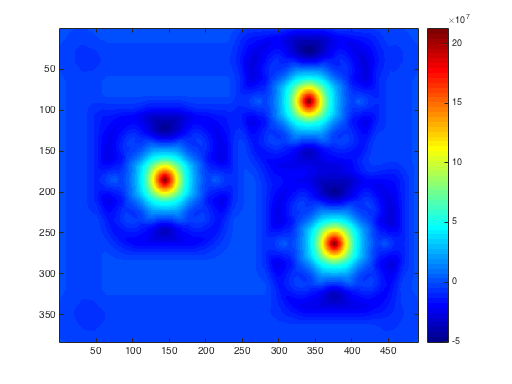
\includegraphics[width=0.45\columnwidth]{4_1_1}
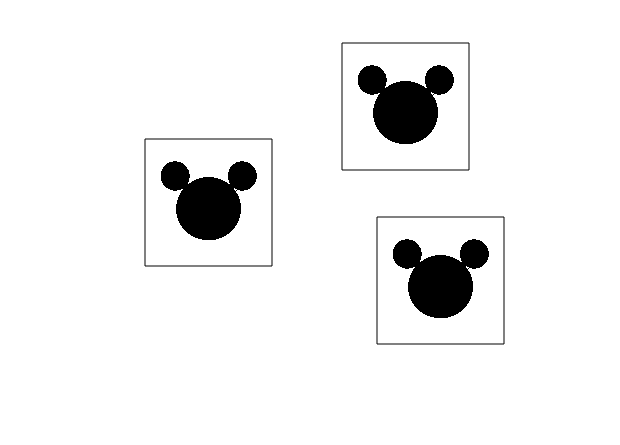
\includegraphics[width=0.45\columnwidth]{4_1_2} \\
\caption{(a) Heat map (b) Bounding boxes}
\label{fig:i4_1}
\end{figure}

Both the filter and the image were really simple in shape and color in this case. However, more realistic images will be more complicated as in shape and color. Unless either the filter or the image are modified, it would be hard to find the most intense locations because there may be too many or none.\\

\item \textbf{Detection Error} : In the previous problem, we implemented the algorithm that produces a bounding box around a detected object. Now, we need to know if the bounding box is good or not. Given a ground truth bounding box ($g$) and a predicted bounding box ($p$), the bounding box quality can be measured by $\frac{p\cap g}{p \cup g}$. Intuitively, this is the number of overlapping pixels between the bounding boxes divided by the total number of unique pixels of the two bounding boxes combined. Assuming that all bounding boxes will be axis-aligned rectangles, we have to implement this error function and try it on the toy example in the previous section. We have to choose 3 different ground truth bounding box sizes around one of the Mickey 3 silhouettes. In general, if the overlap is 50\% or more, the detection did a good job.

\textbf{Solution}

\begin{figure}[H]
\centering
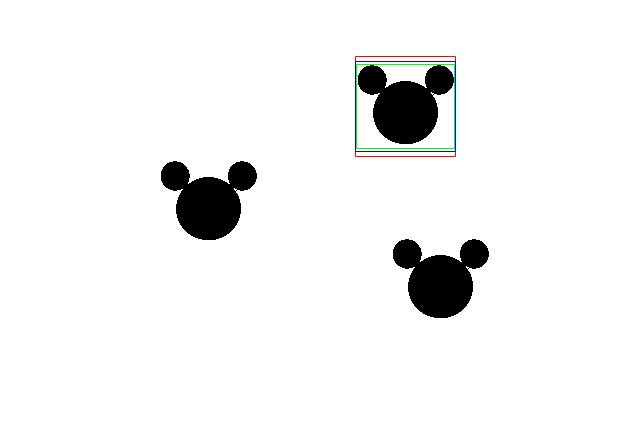
\includegraphics[width=0.8\columnwidth]{4_2}
\caption{Bounding boxes detection in comparison with ground truth}
\label{fig:i4_2}
\end{figure}

For the red groundtruth, the overlap is 0.6404. For the blue groundtruth, the overlap is 0.5767. For the green groundtruth, the overlap is 0.5277. Overall, the performance is good since they are all over 50\%.\\

\item \textbf{More Realistic Images} : We created an algorithm for matching templates and a function to determine the quality of the match. Now, we shift to more realistic images. The file, 'cartemplate.jpg', will be the filter to convolve on each of the 5 other car images ('car1.jpg', 'car2.jpg', 'car3.jpg', 'car4.jpg', 'car5.jpg'). Each image will have an associated text file that contains 2 $(x, y)$ coordinates. These coordinates will be the ground truth bounding box for each image. For each car image, we have to give the following:

\begin{itemize}

\item A heat map image

\item A bounding box drawn on the original image

\item The bounding box overlap percent

\item A description of the pre-processing steps needed to achieve this overlap

\item An explanation of the importance of these steps

\end{itemize}

To formulate the algorithm, we could rescale the car template, rotate it, or blur out the test image/template, or even both.

\textbf {Solution}

\begin{figure}[H]
\centering
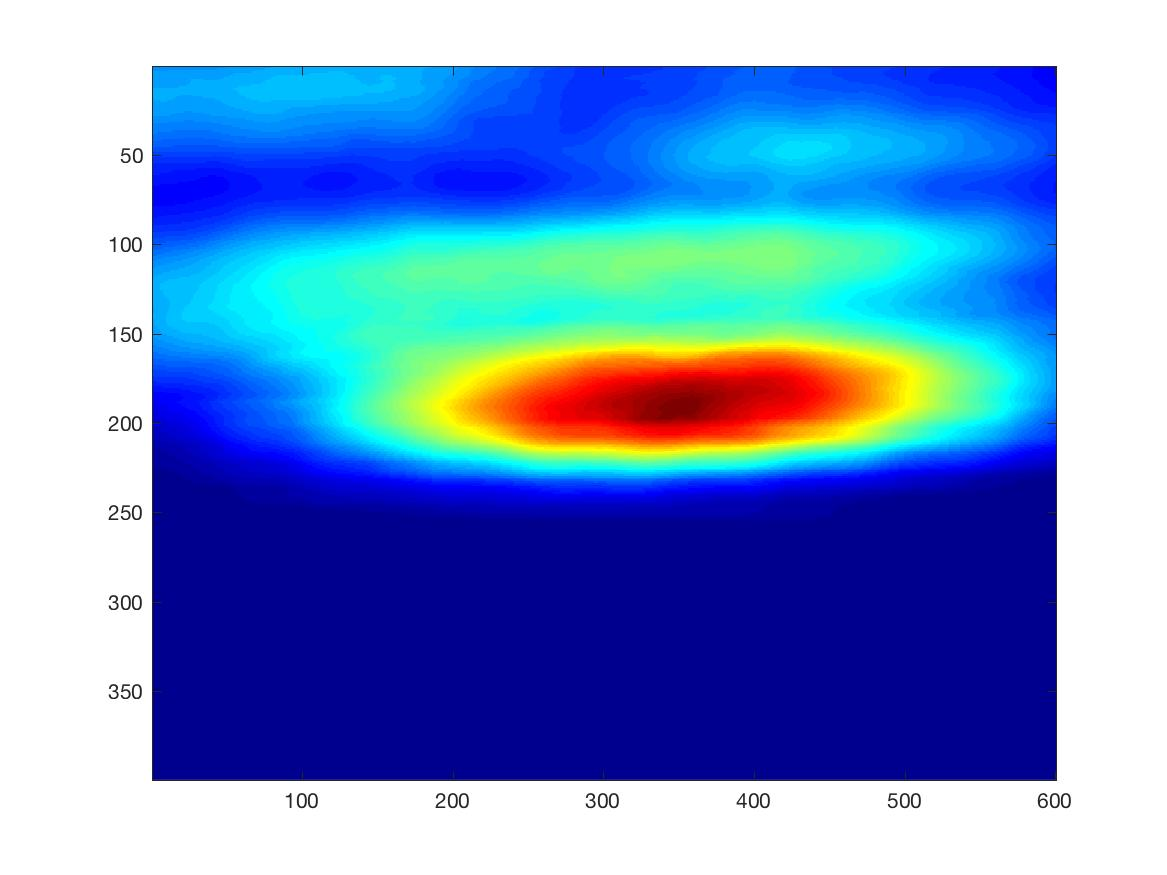
\includegraphics[width=0.4\columnwidth]{9}
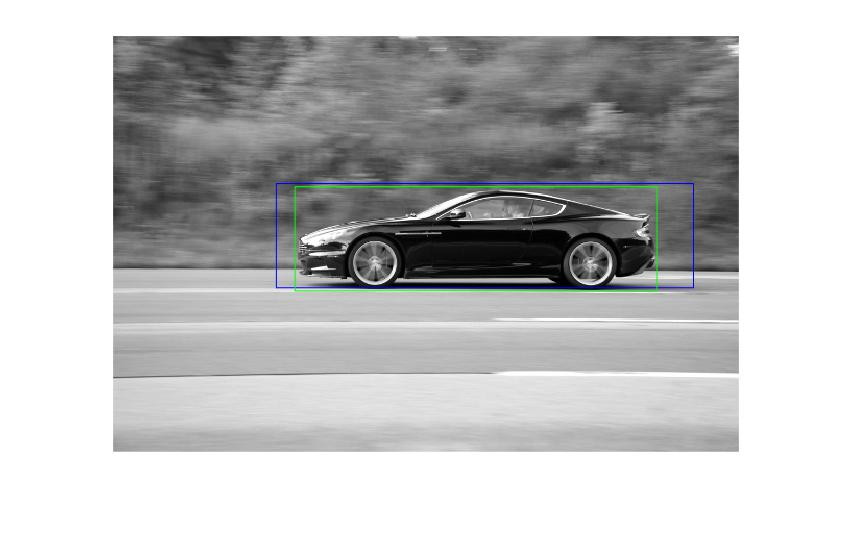
\includegraphics[width=0.4\columnwidth]{9_bbox} \\
\caption{(a) Heat map (b) Bounding box for car 1}
\label{fig:i4_3_1}
\end{figure}

The overlap in the first car is 0.8201. Its quite a straightforward test case as the car is clearly visible and is oriented completely horizontally. The filter was flipped for convolution and resized into a smaller image in order to match the size of the car in the test image. Also both the image and the filter were inversed in color as initially both had dark cars and white surroundings which meant the filter was looking for a similar surrounding rather than a similar car. So to achieve maximum detection we inversed the colors in both so that both cars were in high intensity.

\begin{figure}[H]
\centering
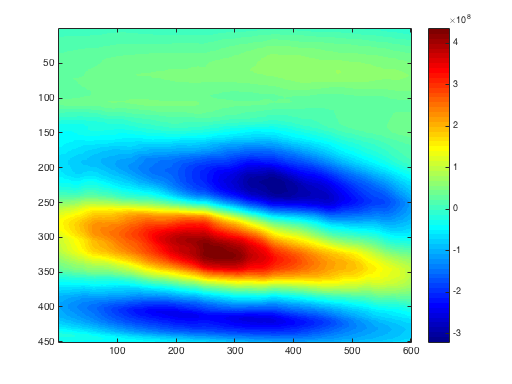
\includegraphics[width=0.4\columnwidth]{4_3_2_1}
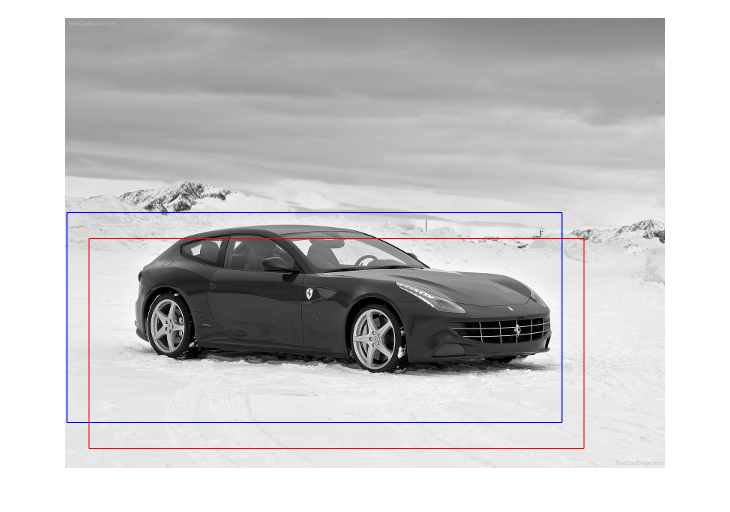
\includegraphics[width=0.4\columnwidth]{4_3_2_2} \\
\caption{(a) Heat map (b) Bounding box for car 2}
\label{fig:i4_3_2}
\end{figure}

We need to flip, rotate, crop, and then resize the car template for the best match. This is because the car in the image is going in the other way and slightly rotated. Also, the car template has blank space which needs to be cropped and it needs to be resized to match that of the image. We designed the algorithm such that it draws a bounding box centered at the averaged position of the maximum intensity values. The overlap is 0.7295.\\

\begin{figure}[H]
\centering
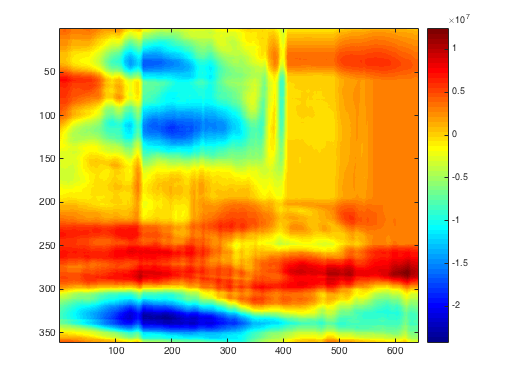
\includegraphics[width=0.4\columnwidth]{4_3_3_1}
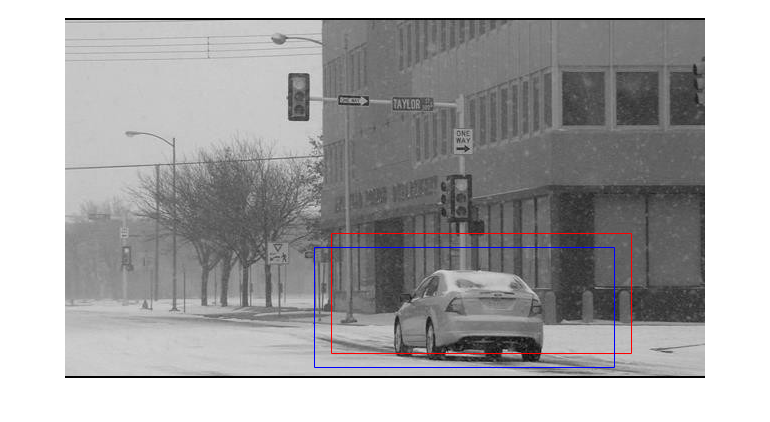
\includegraphics[width=0.4\columnwidth]{4_3_3_2} \\
\caption{(a) Heat map (b) Bounding box for car 3}
\label{fig:i4_3_3}
\end{figure}

We need to inverse the color, fill the dark spots with gray color, rotate, crop, and then resize the car template for the best match. This is because the car in the image if white, rotated, and horizontally smaller. Also, the blank space of the car template needs to be filled with gray or brighter color, because the background of the image is snowy. The same algorithm was used. The overlap is 0.7303.\\

\begin{figure}[H]
\centering
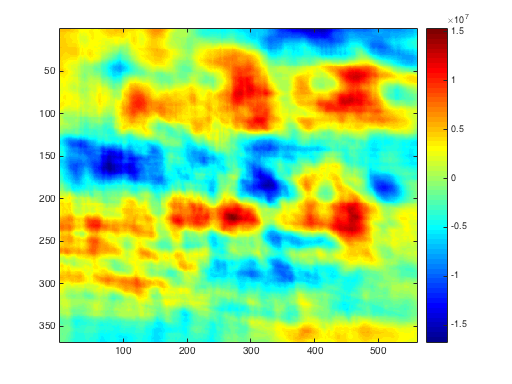
\includegraphics[width=0.4\columnwidth]{4_3_4_1}
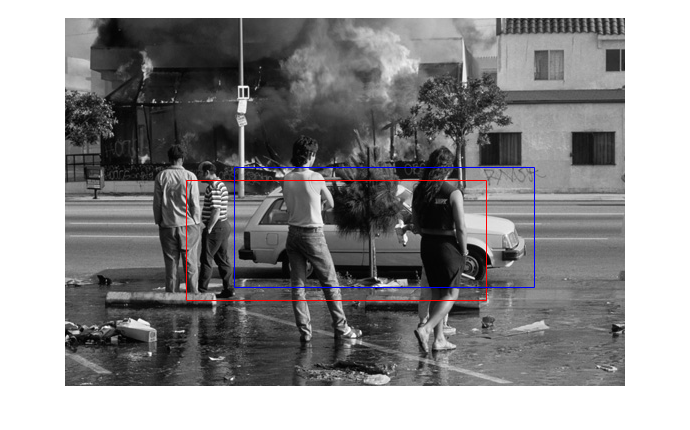
\includegraphics[width=0.4\columnwidth]{4_3_4_2} \\
\caption{(a) Heat map (b) Bounding box for car 4}
\label{fig:i4_3_4}
\end{figure}

We need to flip, inverse the color, fill the dark spots with gray color, crop, and then resize the car template for the best match. This is because the car in the image is going the other way and is white. Also, the car template needs to be cropped and resized to match that in the image. Furthermore, the blank space of the car template needs to be filled with gray or brighter color, because the car is on the gray, asphalt road. The same algorithm was used. The overlap is 0.6116.\\

\begin{figure}[H]
\centering
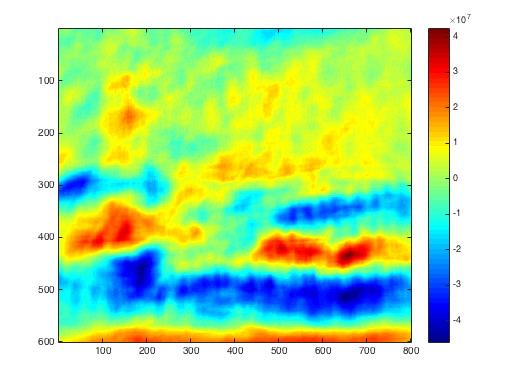
\includegraphics[width=0.4\columnwidth]{4_3_5_1}
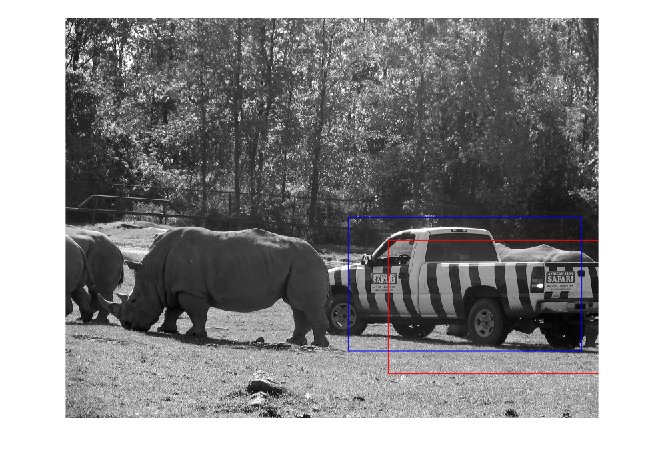
\includegraphics[width=0.4\columnwidth]{4_3_5_2} \\
\caption{(a) Heat map (b) Bounding box for car 5}
\label{fig:i4_3_5}
\end{figure}

We need to inverse the color, fill the dark spots with gray color, crop, and then resize the car template for the best match. This is because the car in the image is going on the other way and the background is composed of trees and grass. Also, the car template needs to be cropped and resized to match that of the image. The same algorithm was used. The overlap is 0.5317.\\

\item \textbf{Invariance} : The detection algorithm that was implemented for this problem may have seemed a bit brittle. We have to describe a few things that this algorithm was not invariant to. 

\textbf{Solution}

The filter was also not invariant to the color the of the car. Plain colored cars like the first image was easy to detect unlike the last one which had stripes.
It depended upon the shape of the car. As again the first car matched pretty well whereas the last one wasn't the same shape as the template and hence had difficulties.
The occulusion level also affected the detection as template matching solely depends on matching two given windows. Occlusions cover up the object being matched.
The algorithm is not invariant to the orientation of the car. It needs to use a differently oriented filter for each image depending upon the orientation of the car in that image.


\end{enumerate}

\pbitem \textbf{Canny Edge Detection} : This problem requires us to implement a function to perform Canny Edge Detection. The steps to be followed are:

\begin{itemize}

\item \textbf{Smoothing} : Smoothing is required to remove noise from being considered edges. We have to use a $5 \times 5$ Gaussian kernel filter with $\sigma = 1.4$ to smooth the images.

\begin{equation}
K = \frac{1}{159}\begin{bmatrix}
2 & 4 & 5 & 4 & 2 \\
4 & 9 & 12 & 9 & 4 \\
5 & 12 & 15 & 12 & 5 \\
4 & 9 & 12 & 9 & 4 \\
2 & 4 & 5 & 4 & 2 \\
\end{bmatrix}
\end{equation}

\item \textbf{Gradient Computation} : We have to find the image gradient in the horizontal and vertical directions. We can use Sobel operators as filter kernel to calculate $G_x$ (gradient along the x-axis) and $G_y$ (gradient along the y-axis). $s_x$ and $s_y$ are the corresponding kernels. We have to compute the gradient magnitude image as $|G| = \sqrt[]{G_x^2 + G_y^2}$. The edge direction at each pixel is given by $G_\theta = tan^{-1}(\frac{G_y}{G_x})$.

\begin{equation}
s_x = \begin{bmatrix}
-1 & 0 & 1 \\
-2 & 0 & 2 \\
-1 & 0 & 1 \\
\end{bmatrix},
s_y = \begin{bmatrix}
-1 & -2 & -1 \\
0 & 0 & 0 \\
1 & 2 & 1 \\
\end{bmatrix}
\end{equation}

\item \textbf{Non maximum suppression} : The desired edges need to be sharp. So, we are required to use non-maximum suppression to preserve the local maxima and discard the rest. The method we will follow is:

For every pixel,

\begin{itemize}

\item Round off the gradient direction $\theta$ to the nearest multiple of $45\deg$ in a 8-connected neighborhood. 

\item Compare the edge strength at the current pixel to the pixels along the positive and negative gradient direction in the 8-connected neighbourhood.

\item Preserve the values of only those pixels which have maximum gradient magnitudes in the neighbourhood along the +ve and −ve gradient direction.

\end{itemize}

\item \textbf{Hysteresis Thresholding} : 

\end{itemize}

We have to compute the images at each step and select thresholds that retain most of the true edges. The image to be used is 'geisel.jpg'.

\textbf{Solution}

\begin{figure}[H]
\centering
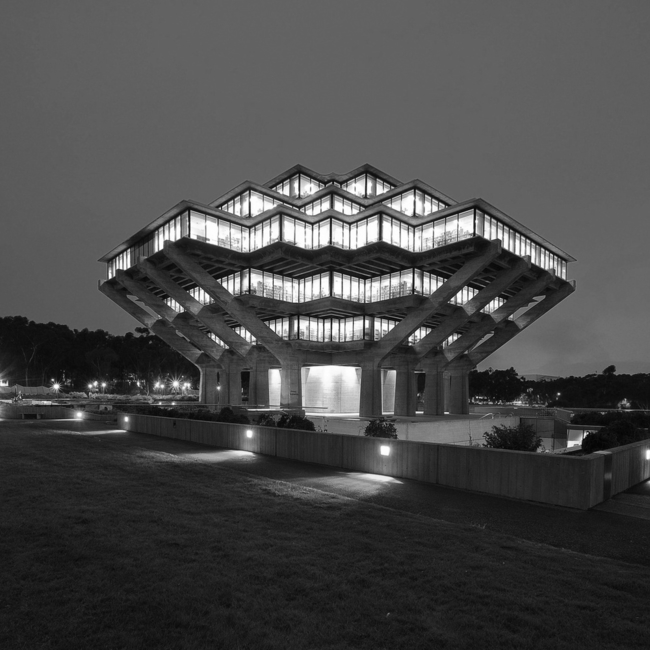
\includegraphics[width=0.3\columnwidth]{geisel}
\caption{Original image}
\label{fig:i5}
\end{figure}

\begin{figure}[H]
\centering
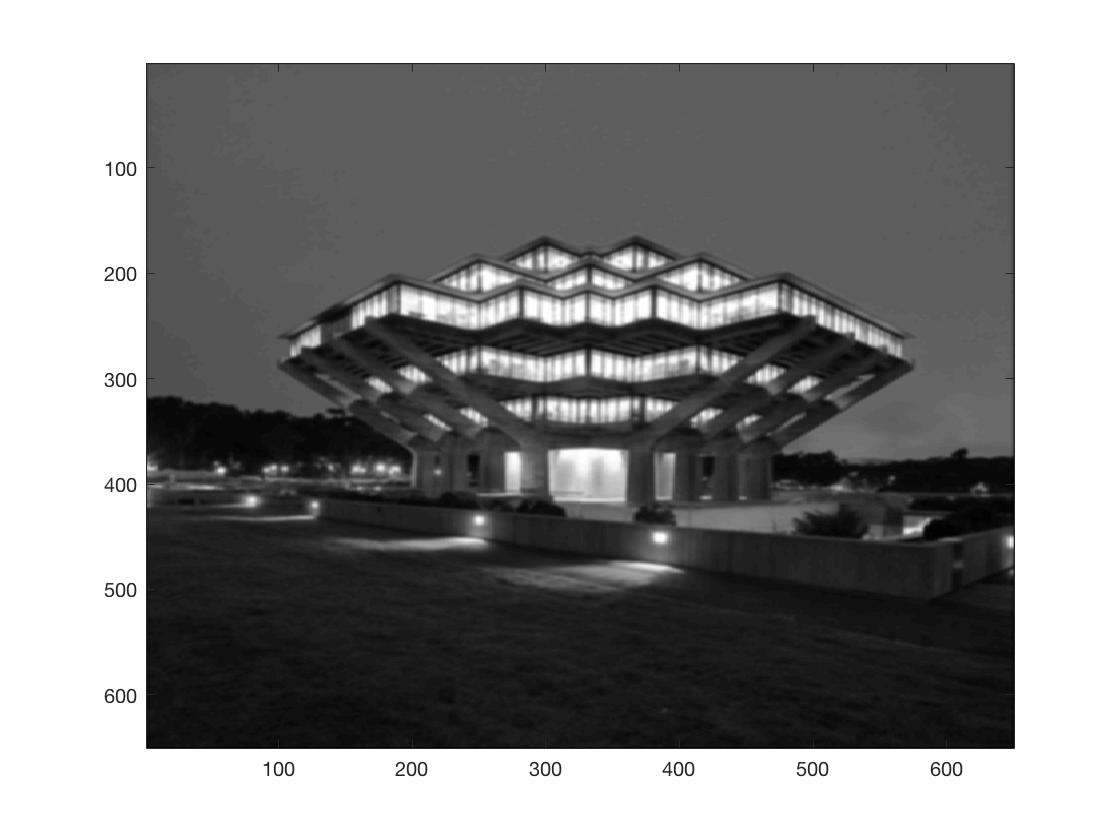
\includegraphics[width=0.4\columnwidth]{5_2}
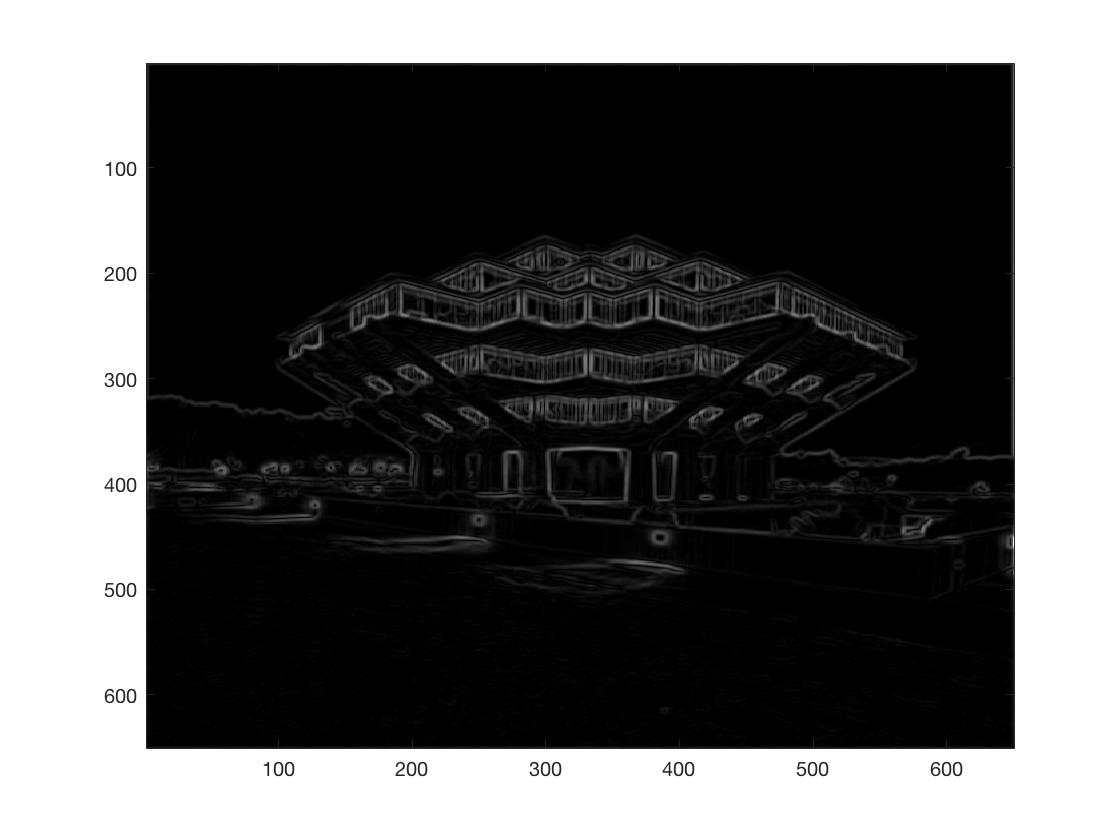
\includegraphics[width=0.4\columnwidth]{5_3} \\
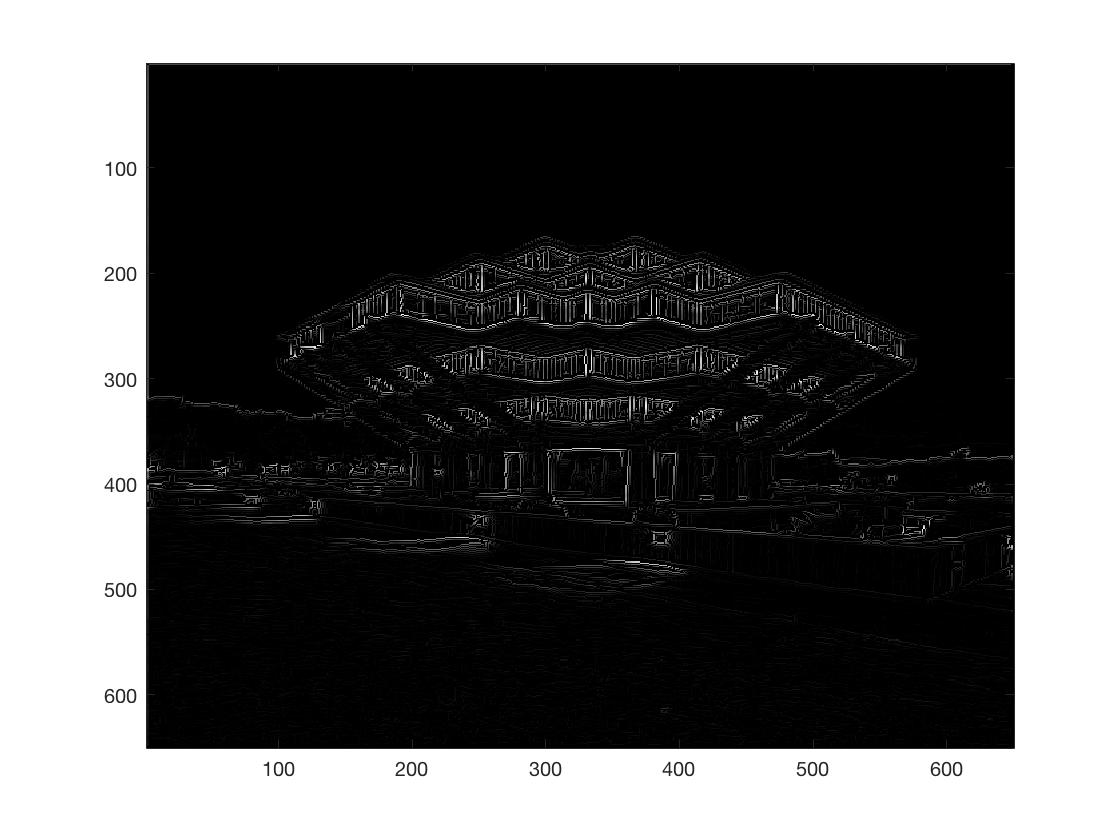
\includegraphics[width=0.4\columnwidth]{5_4}
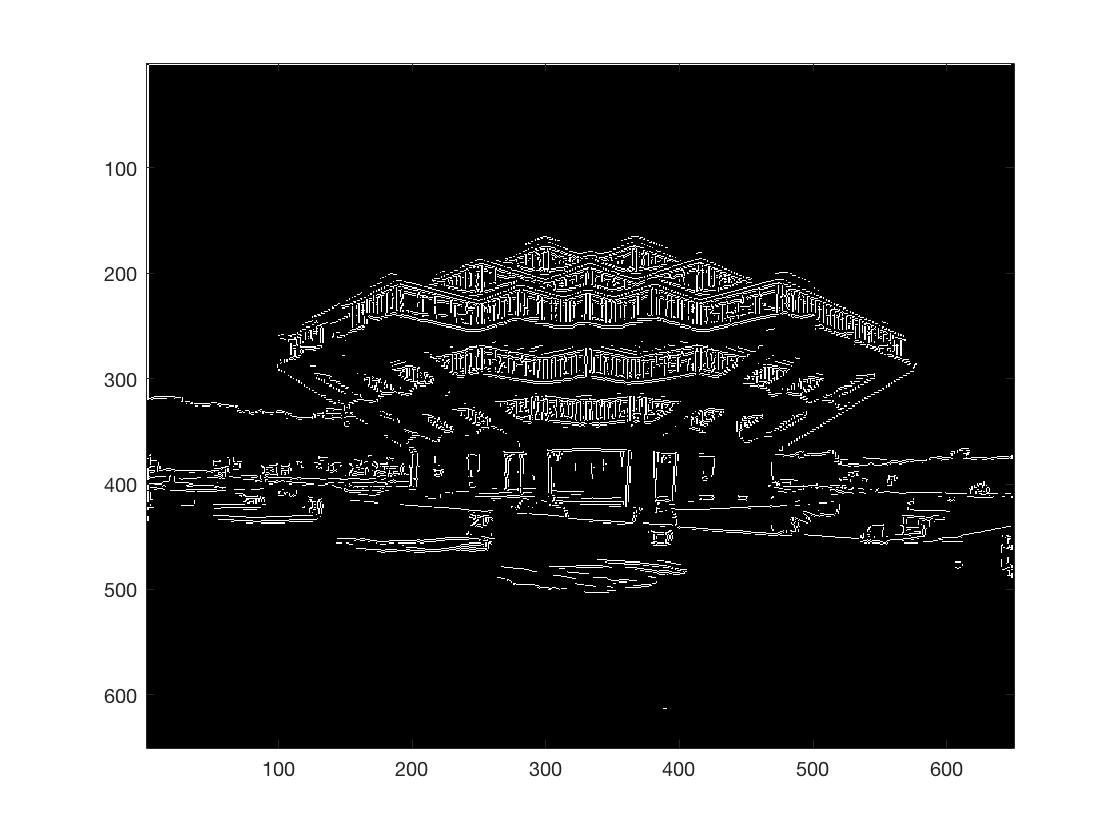
\includegraphics[width=0.4\columnwidth]{5_5}
\caption{(a) Smoothed Image (b) Gradient Magnitude (c) NMS edges (d) Final edges after thresholding}
\label{fig:i5_1}
\end{figure}

The optimal threshold values were obtained by using an upper threshold of 40 and a lower threshold of 20.

\pbitem \textbf{Sparse Stereo Matching} : We are given two figures, 'warrior2.mat' and 'matrix2.mat'. These files contain two images, two camera matrices and sets of corresponding points extracted by manually clicking on the images. 

\begin{enumerate}[label*=\arabic*.]

\item \textbf{Corner Detection} : We have to build a corner detector. The file should be named 'CornerDetect.m' and should take in as input the following arguments:

\begin{verbatim}

corner = CornerDetect(Image, nCorners, smoothSTD, windowSize)

\end{verbatim}

Here, 

\begin{itemize}

\item smoothSTD = standard deviation of the smoothing kernel

\item windowSize = size of the smoothing window

\item nCorners = number of strongest corners to be returned after non-maximum suppression (Here, we will use nCorners = 20)

\end{itemize}

\textbf{Solution}

\begin{figure}[H]
\centering
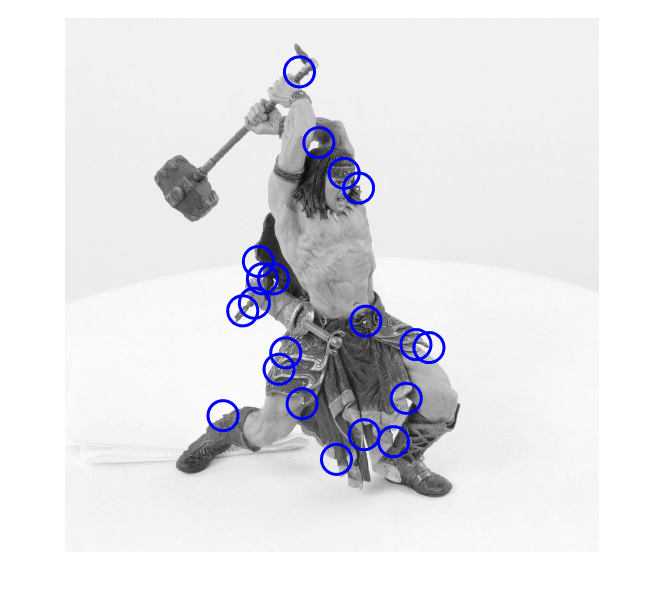
\includegraphics[width=0.4\columnwidth]{w6_1_1}
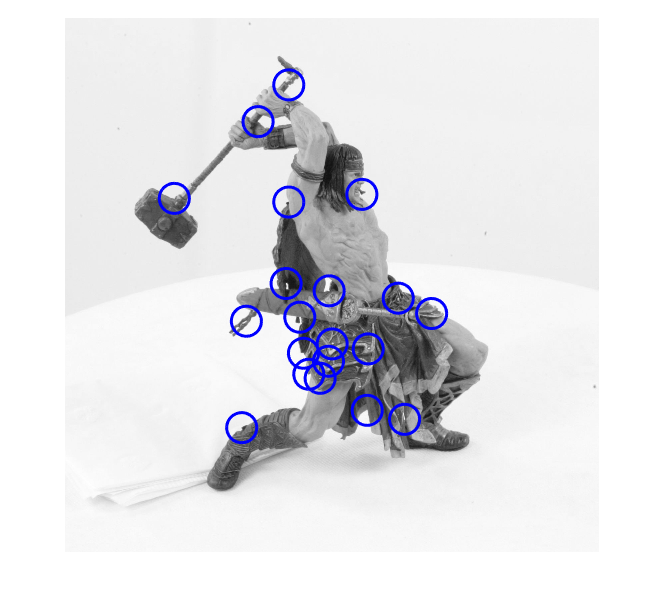
\includegraphics[width=0.4\columnwidth]{w6_1_2} \\
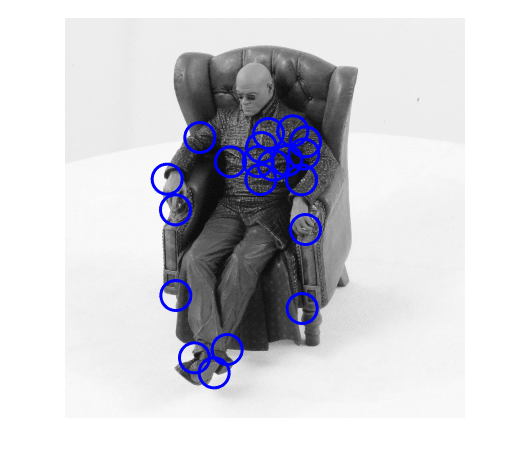
\includegraphics[width=0.4\columnwidth]{m6_1_1}
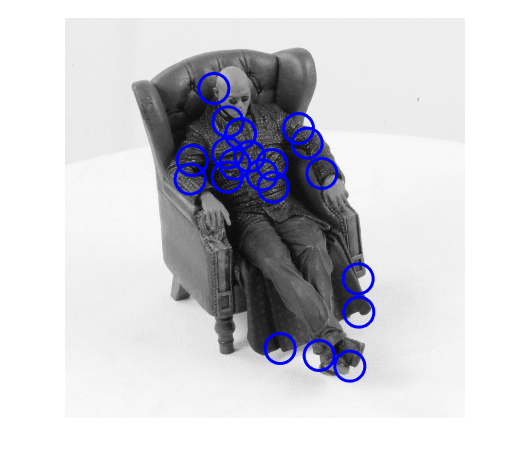
\includegraphics[width=0.4\columnwidth]{m6_1_2}
\caption{(a) Warrior Image 1 (b) Warrior Image 2 (c) Matrix Image 1 (d) Matrix Image 2}
\label{fig:i6_1}
\end{figure}

Reference the appendix for the values used for nCorners, smoothSTD, and windowSize.\\

\item \textbf{SSD Matching} : We have to write a function that implements the SSD matching algorithm for two input windows.

\textbf{Solution}

Reference the appendix for the values used for the size of the patches for SSD comparison.\\

\item \textbf{Naive Matching} : We have to now find correspondences. we will start with trying to find the best match between two sets of corner points. For each corner in image1, we have to find the best match from the detected corners in image2. If the SSD match score is very low, there is no match for that point. We have to find a good threshold value. We have to write a function 'naiveCorrespondenceMatching.m' and use it in the following way:

\begin{verbatim}
ncorners = 10;
corners1 = CornerDetect(I1, ncorners, smoothSTD, windowSize));
corners2 = CornerDetect(I2, ncorners, smoothSTD, windowSize));
[I, corsSSD] = naiveCorrespondenceMatching(I1, I2, corners1, corners2, 
R, SSDth);
\end{verbatim}

\textbf{Solution}

\begin{figure}[H]
\centering
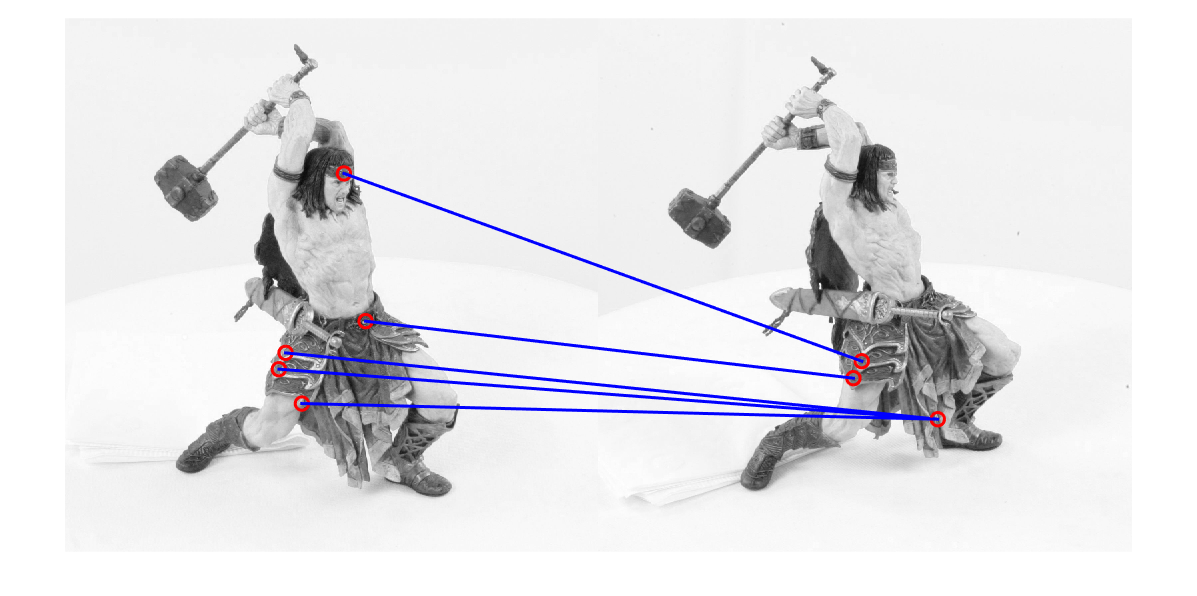
\includegraphics[width=0.9\columnwidth]{w6_3} \\
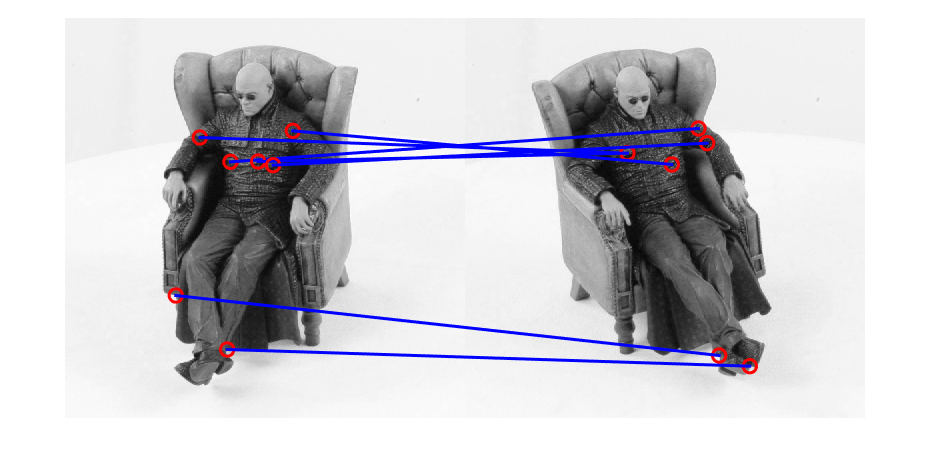
\includegraphics[width=0.95\columnwidth]{m6_3} 
\caption{(a) Warrior Image (b) Matrix Image}
\label{fig:i6_3}
\end{figure}

Reference the appendix for values used for nCorners, smoothSTD, windowSize, R, and SSDth. In general, the matching is terrible. When you look at the matched corners closely, they kind of resemble each other as in color and shape. However, the actual locations of the corners were not considered, so many corners from the left image were matched to corners in totally different places in the right image.\\

\item \textbf{Epipolar Geometry} : We have to use the file 'fund.m' and the provided points cor1 and cor2, to calculate the fundamental matrix and plot the epipolar lines in both image pairs. We could use 'linePts.m'.

\textbf{Solution}

\begin{figure}[H]
\centering
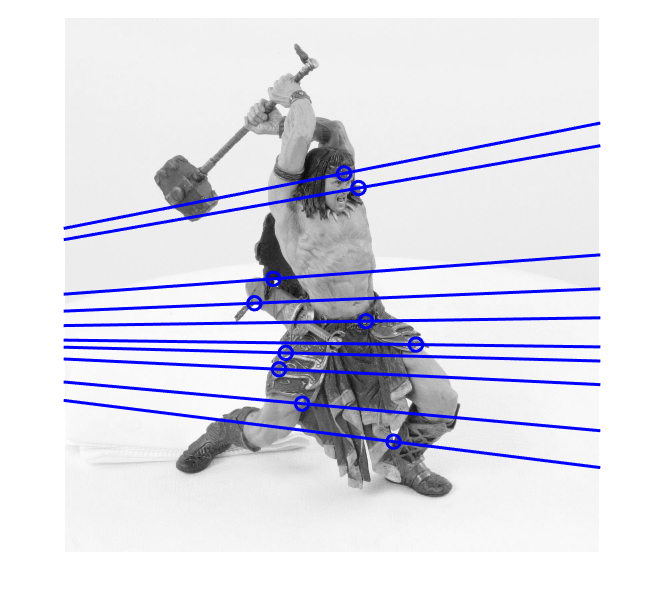
\includegraphics[width=0.45\columnwidth]{w6_4_1}
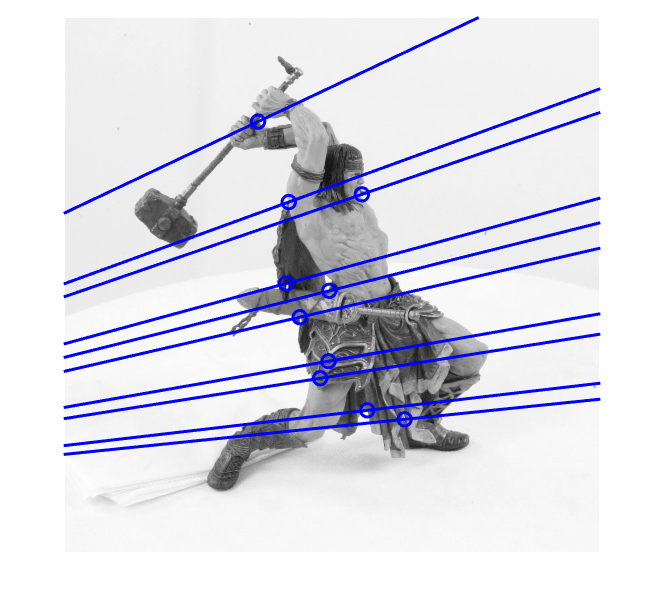
\includegraphics[width=0.45\columnwidth]{w6_4_2} \\
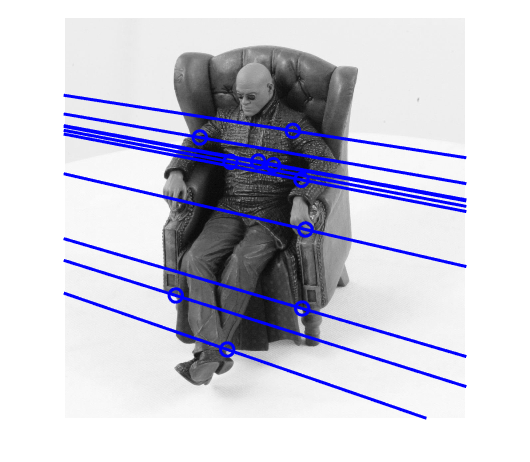
\includegraphics[width=0.45\columnwidth]{m6_4_1}
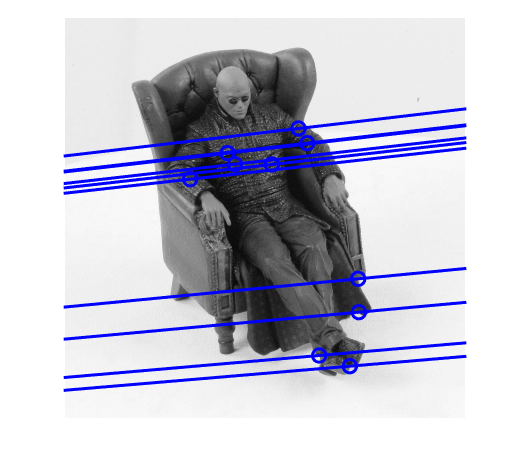
\includegraphics[width=0.45\columnwidth]{m6_4_2}
\caption{(a) Warrior Image 1 (b) Warrior Image 2 (c) Matrix Image 1 (d) Matrix Image 2}
\label{fig:i6_4}
\end{figure}

The epipolar lines for the warrior images look like they are running in the similar way, while the epipolar lines for the matrix images look like they are running in the opposite way. This is, presumably, because the pictures of the warrior were taken at camera positions with relatively small angle variation, while the pictures of the matrix figure were taken at camera positions with relatively large angle variation.\\

\item \textbf{Epipolar Geometry Based Matching} : We will now build a better matching algorithm using epipolar geometry. We first have to detect 10 corners in image1, and for each corner, do a linesearch along the corresponding epipolar line in image2. We then evaluate the SSD score for each point along this line and return the best match, or no match if the scores are too low. R is the radius of the SSD patch.


\begin{verbatim}
ncorners = 10;
F = fund(cor1, cor2);
corners1 = CornerDetect(I1, ncorners, smoothSTD, windowSize));
corsSSD = correspondenceMatchingLine( I1, I2, corners1, F, R, SSDth);
\end{verbatim}

\textbf{Solution}

\begin{figure}[H]
\centering
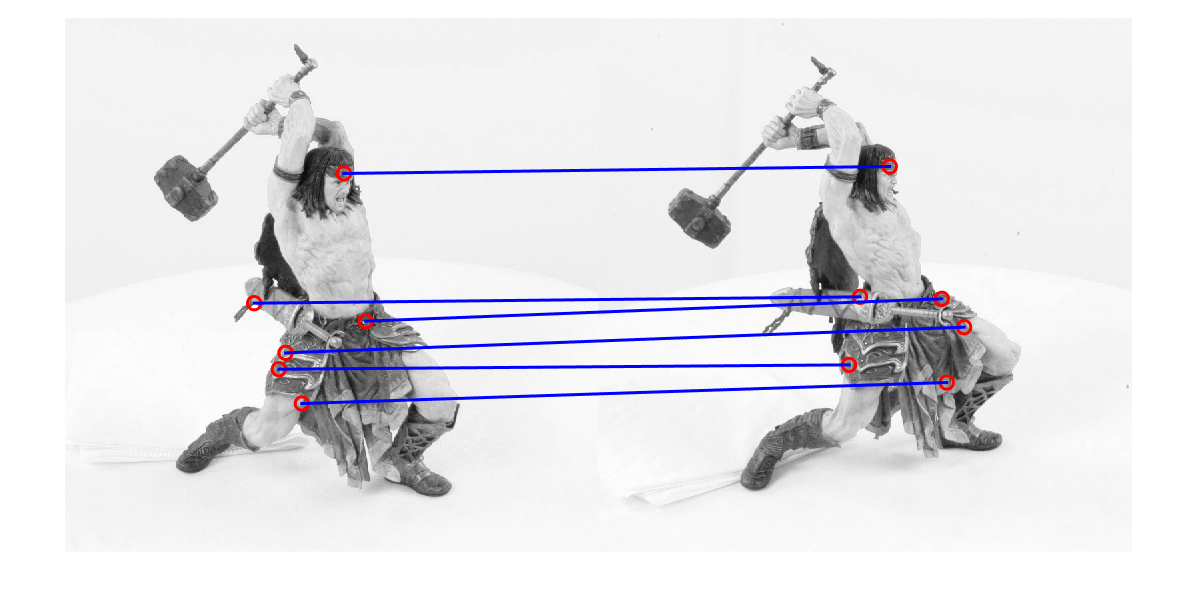
\includegraphics[width=0.9\columnwidth]{w6_5} \\
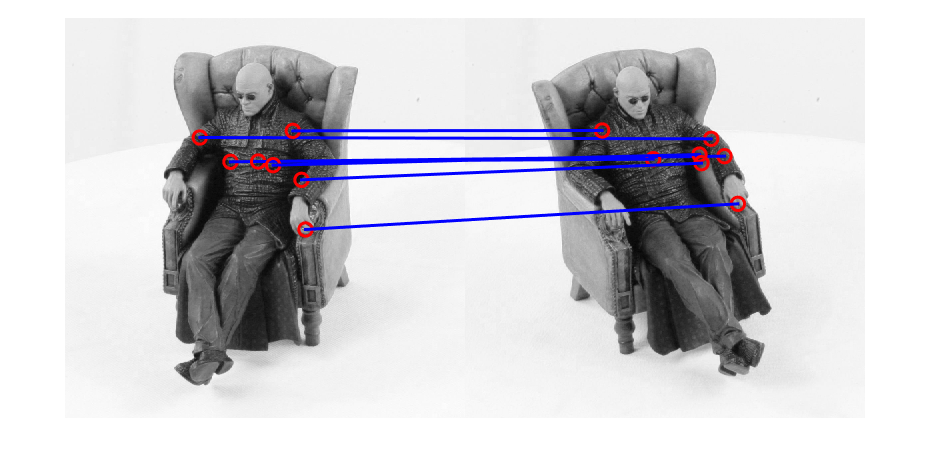
\includegraphics[width=0.9\columnwidth]{m6_5} 
\caption{(a) Warrior Image (b) Matrix Image}
\label{fig:i6_5}
\end{figure}

Now the matching is significantly better than that of 6.3. However, there are still mismatched corners. Using epipolar geometry prevents the corners from being mapped to a totally different positions(e.g. head to foot or arm to foot), but it can result in matching similar looking corners given that they are on the same epipolar line, as you can see in Figure 13(b).\\

\item \textbf{Triangulation} : After we have found the correspondences between the pairs of images, we can now proceed to the triangulation of the corresponding 3-D points. The correspondences may contain noise and many outliers as we have not enforced the ordering constraint. We have to triangulate a 3-D point for each corresponding pair of points using the provided camera matrices. P1 and P2 are the camera matrices. We also have to write a function 'findOutliers.m' that reprojects the world points to image2 and then deterines which points are outliers and inliers. We will call a point an outlier if the distance between the true location, and the reprojected point location is more than 20 pixels.

\begin{verbatim}
outlierTH = 20;
F = fund(cor1, cor2);
ncorners = 50;
corners1 = CornerDetect(I1, ncorners, smoothSTD, windowSize));
corsSSD = correspondanceMatchingLine( I1, I2, corners1, F, R, SSDth);
points3D = triangulate(corsSSD, P1, P2);
[ inlier, outlier ] = findOutliers(points3D, P2, outlierTH, corsSSD);
\end{verbatim}

The results should be displayed as:

\begin{itemize}

\item original points - black circles

\item inliers - blue plus points

\item outliers - red plus signs

\end{itemize}

Do the detected outliers correspond to false matches?

\textbf{Solution}

The occurrence of outliers may be due to the inaccuracies in feature detection, false matching, and several errors in the estimation of fundamental matrices and projection matrices. A common source of error is mismatches satisfying the epipolar constraint by coincidence, which in turn lead to the reconstruction of erroneous 3D points that yield small reprojection errors.

\begin{figure}[H]
\centering
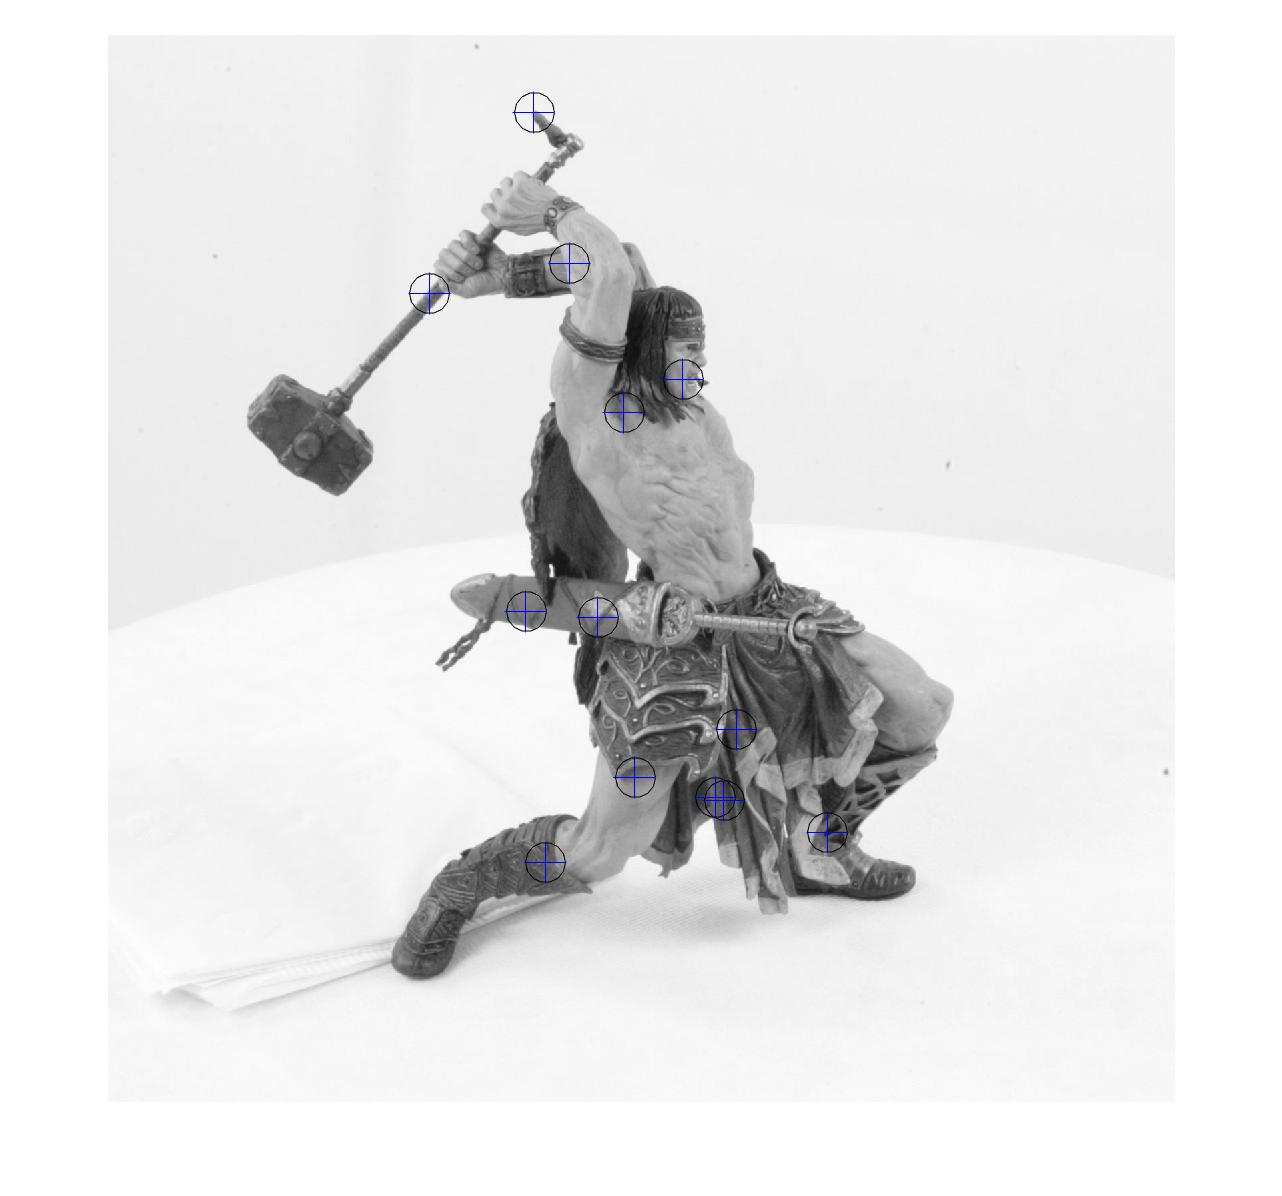
\includegraphics[width=0.45\columnwidth]{6_6_warrior}
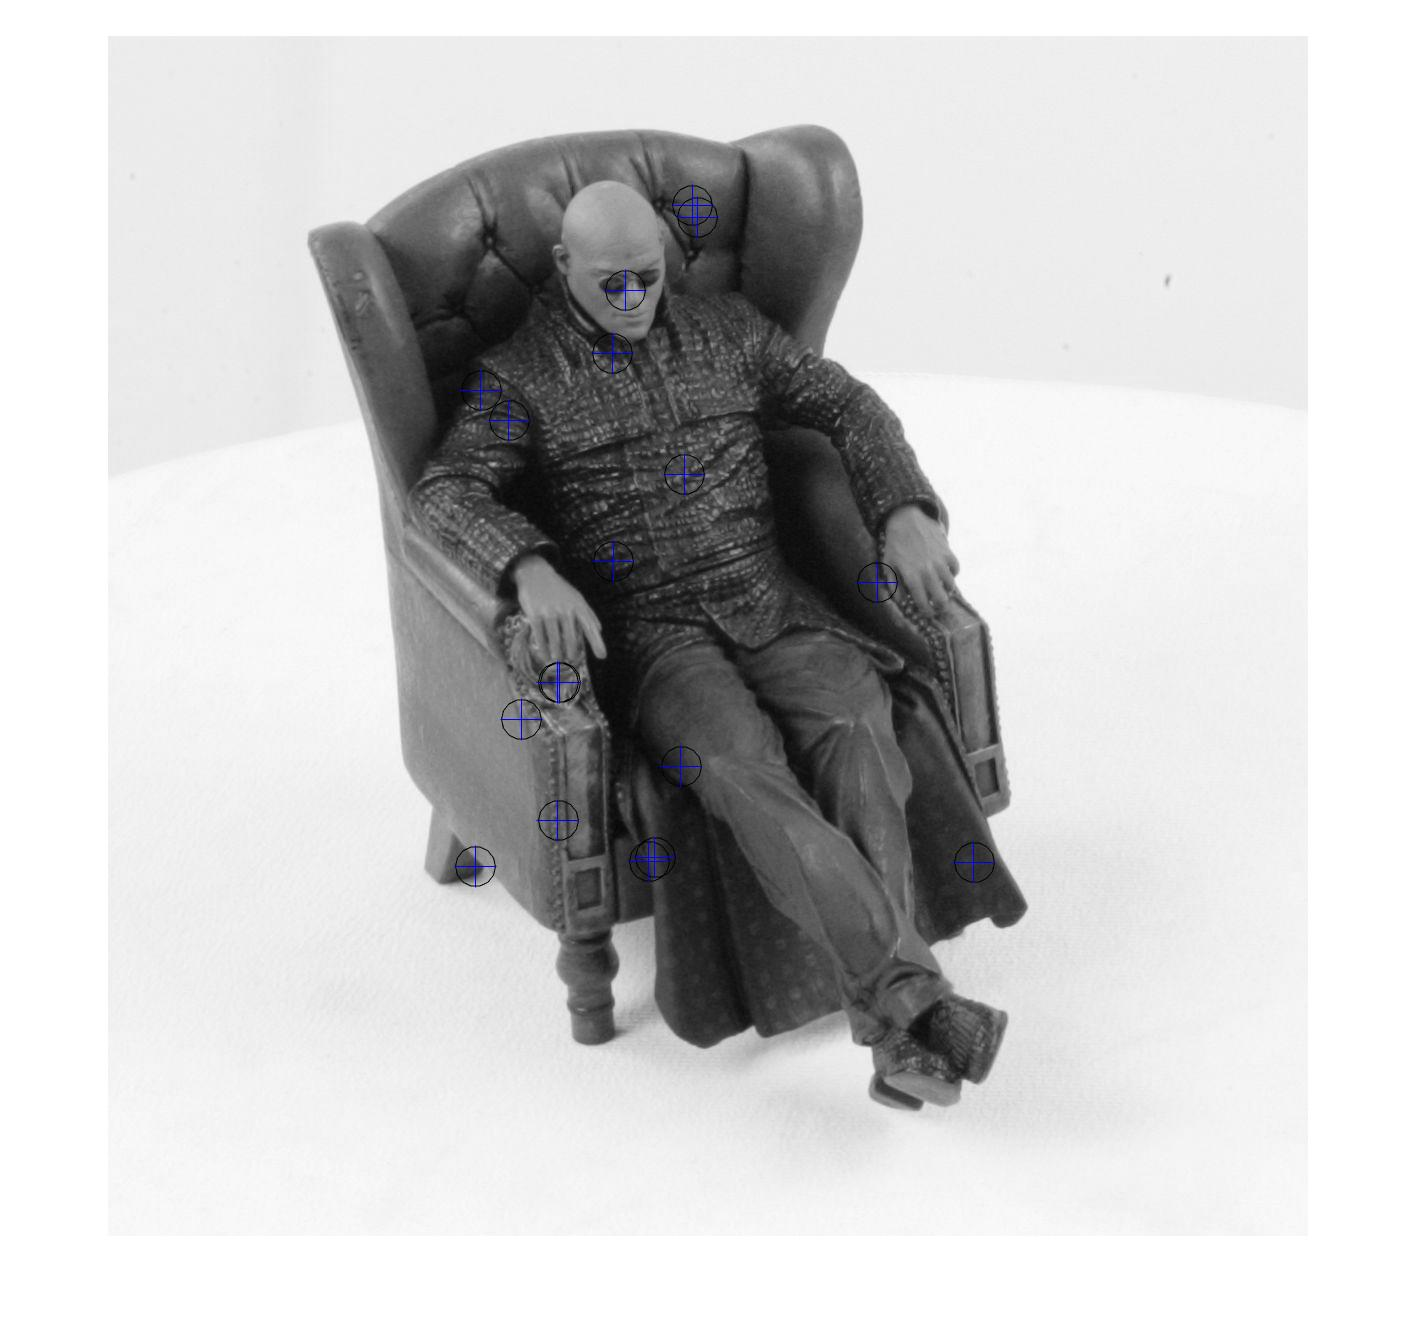
\includegraphics[width=0.45\columnwidth]{6_6_matrix} 
\caption{(a) Warrior Image (b) Matrix Image}
\label{fig:i6_5}
\end{figure}

\end{enumerate}

\end{problemlist}

\section*{Appendix}

\lstinputlisting[language=MATLAB, caption=MATLAB source for 4.1]{4_1_.m}
\lstinputlisting[language=MATLAB, caption=MATLAB source for 4.2]{4_2_.m}
\lstinputlisting[language=MATLAB, caption=MATLAB source for 4.3]{4_3_.m}
\lstinputlisting[language=MATLAB, caption=MATLAB source for 4.3(car 1)]{q4_3_2.m}
\lstinputlisting[language=MATLAB, caption=MATLAB source for error function]{error_func.m}
\lstinputlisting[language=MATLAB, caption=MATLAB source for conv function]{conv_func.m}
\lstinputlisting[language=MATLAB, caption=MATLAB source for 5]{q5.m}
\lstinputlisting[language=MATLAB, caption=MATLAB source for 6.1]{CornerDetect.m}
\lstinputlisting[language=MATLAB, caption=MATLAB source for 6.2]{SSDmatch.m}
\lstinputlisting[language=MATLAB, caption=MATLAB source for 6.3]{naiveCorrespondanceMatching.m}
\lstinputlisting[language=MATLAB, caption=MATLAB source for 6.4]{problem6.m}
\lstinputlisting[language=MATLAB, caption=MATLAB source for 6.5]{correspondanceMatchingLine.m}
\lstinputlisting[language=MATLAB, caption=MATLAB source for 6.6]{q6_6.m}
\lstinputlisting[language=MATLAB, caption=MATLAB source code for findOutliers function]{findOutliers.m}
\lstinputlisting[language=MATLAB, caption=MATLAB source for triangulate function]{triangulate.m}
\lstinputlisting[language=MATLAB, caption=MATLAB source for fund function]{fund.m}
\lstinputlisting[language=MATLAB, caption=MATLAB source for linePts function]{linePts.m}

\end{document}
